\documentclass[10pt,aspectratio=169]{beamer}
\usetheme[progressbar=frametitle,numbering=fraction]{metropolis}
\usepackage[T1]{fontenc}
\usepackage{booktabs}
\usepackage{multirow}
\usepackage{xspace}

\newcommand{\qwen}{Qwen2.5-VL-7B\xspace}
\newcommand{\llava}{LLaVA-NeXT-7B\xspace}
\newcommand{\cls}[1]{\MakeUppercase{#1}}
\newcommand{\hl}[1]{\alert{\textbf{#1}}}
\setbeamerfont{footnote}{size=\tiny}

\title{Type-Aware Failure Prediction for Chart Reasoning in VLMs}
\subtitle{Mid-term status, for TA guidance}
\author{Yash More \and Naman Singhal \and Shrish Kadam \and Sanjith Ganapathi}
\institute{ANLP course project, IIIT Hyderabad}
\date{30 September 2026}

\begin{document}

\maketitle

% ---------------------------------------------------------------------------
\section{The question}

\begin{frame}{Two ways to answer a chart question wrongly}
\begin{columns}[T]
\column{0.48\textwidth}
\textbf{Structural failure (misread)}
\begin{itemize}
\item Wrong bar, misjudged tick, miscounted slices
\item The answer \emph{is} in the image
\item Repair: look again (crop, re-ask)
\end{itemize}
\column{0.48\textwidth}
\textbf{Fabrication}
\begin{itemize}
\item States a value or label the chart does not contain
\item Looking again cannot help
\item Repair: abstain
\end{itemize}
\end{columns}
\vspace{1em}
Today's reliability tools collapse both into one ``do not trust'' score.
\vspace{0.5em}

\hl{Type Separability Hypothesis:} the model's internal state \emph{before} it
answers is linearly different for a coming misread and a coming fabrication.
A collapse of the two into one signal is a reportable outcome, not a failure.
\end{frame}

\begin{frame}{Experiments at a glance}
\begin{tabular}{lp{0.72\textwidth}l}
\toprule
& What it asks & Status \\
\midrule
E1 & Can a probe predict \emph{whether} the answer will be wrong? & done \\
E2 & Is the probe just reading surface features of the input? & partial \\
E3 & Are the misread and fabrication signals different (cross-transfer)? & done (synthetic) \\
E4 & Does the failure type decide which repair works? & code ready \\
E5 & A controller that picks the repair from the probes & Oct \\
\bottomrule
\end{tabular}
\vspace{1em}

Two data arms: \textbf{ChartQA} (real charts, naturally occurring errors) and a
\textbf{synthetic bar-chart arm} (errors induced on purpose).
\end{frame}

% ---------------------------------------------------------------------------
\section{Pipeline}

\begin{frame}{Setup}
\begin{columns}[T]
\column{0.5\textwidth}
\textbf{Models} (frozen, fp16, greedy)
\begin{itemize}
\item \qwen (28 layers, $d=3584$)
\item \llava, Mistral LM (32 layers, $d=4096$)
\item ChartGemma dropped
\end{itemize}
\textbf{Data}
\begin{itemize}
\item ChartQA test: 2,500 questions (1,250 human, 1,250 augmented)
\item ChartQA val\_human: 960 (Qwen)
\item Two synthetic pilots: 2,400 questions
\end{itemize}
\column{0.5\textwidth}
\textbf{Activations}
\begin{itemize}
\item Forward hooks inside the \emph{same} \texttt{generate()} call that produced
the labelled answer
\item Every layer, 4 pooled positions: image-token mean/max, last prompt token,
prompt mean
\end{itemize}
\textbf{Probes}
\begin{itemize}
\item $L_2$ logistic regression on one vector, scored by AUROC
\item Splits by \emph{chart}, never by question
\item Figure-level bootstrap CIs
\item Always next to a baseline that sees no activations
\end{itemize}
\end{columns}
\end{frame}

% ---------------------------------------------------------------------------
\section{Naturalistic arm: ChartQA}

\begin{frame}{Accuracy}
\centering
\begin{tabular}{lccc}
\toprule
Model & Overall & Human & Augmented \\
\midrule
\qwen & 87.3 & 79.8 & 94.8 \\
\llava & 52.9 & 44.6 & 61.1 \\
\bottomrule
\end{tabular}
\vspace{1em}

Relaxed accuracy (\%), numeric within 5\% of gold.\\
Qwen is wrong on \textbf{317} questions, LLaVA on \textbf{1,178}.
\end{frame}

\begin{frame}{What Qwen's 317 errors actually are}
\begin{columns}[T]
\column{0.46\textwidth}
\begin{tabular}{lr}
\toprule
Label & $n$ \\
\midrule
\cls{not\_an\_error} & 112 \\
\cls{computation} & 93 \\
\cls{structural} & 71 \\
\cls{ambiguous} & 40 \\
\cls{fabrication} & \hl{1} \\
\bottomrule
\end{tabular}
\vspace{0.5em}

\footnotesize Labelled by an LLM annotator (Claude Opus 5.5) that saw only
image, question, gold and answer, following a written rubric. Human
agreement check not yet run.
\column{0.52\textwidth}
\begin{itemize}
\item \hl{Fabrication is essentially absent} from ChartQA: questions are
written about content the chart contains
\item \hl{35\% are not errors}: equivalent format, wrong gold, or a valid
reading of the question
\item \cls{computation} (inputs read right, arithmetic wrong) is the
\hl{largest real class}; the proposal's two-class taxonomy had no slot for it
\end{itemize}
$\Rightarrow$ ChartQA cannot supply fabrication examples. This is why the
synthetic arm exists.
\end{columns}
\end{frame}

\begin{frame}{Label noise in ChartQA itself}
\begin{columns}[T]
\column{0.5\textwidth}
\begin{tabular}{lcc}
\toprule
& Human & Augmented \\
\midrule
Questions & 1250 & 1250 \\
Scored wrong & 252 & 65 \\
Real errors & 140 & 25 \\
Gold answer wrong & 16 & \hl{18} \\
\bottomrule
\end{tabular}
\column{0.48\textwidth}
\begin{itemize}
\item 34 of 317 gold answers are wrong; on augmented questions that is
28\% of the ``errors''
\item 16 answers are the right number on the other scale (0.43 for a gold of
43): the metric scores them wrong
\item Counting those as correct: 87.3\% $\to$ 88.0\%; counting all
\cls{not\_an\_error}: 91.8\%
\end{itemize}
\end{columns}
\vspace{0.8em}
Every probe trained on relaxed-accuracy labels inherits this noise.
\end{frame}

\begin{frame}{E1: predicting whether the answer will be wrong}
\centering
\begin{tabular}{lcc}
\toprule
Test AUROC [95\% CI] & Probe & Surface baseline \\
\midrule
Qwen, all errors & 0.877 {\scriptsize[.83, .92]} & 0.715 \\
Qwen, without \cls{not\_an\_error} & \hl{0.932} {\scriptsize[.90, .96]} & 0.786 \\
LLaVA, all errors & 0.798 {\scriptsize[.76, .84]} & 0.608 \\
\midrule
Qwen, structural vs.\ correct & 0.905 {\scriptsize[.84, .97]} & -- \\
\bottomrule
\end{tabular}
\vspace{0.8em}
\raggedright
\begin{itemize}
\item Surface baseline: question source, length, image tokens, numeric gold
\item Removing label noise \emph{raises} the probe: part of its ``error'' was
the labels
\item Not just question style: within human-written questions only, 0.895
(Qwen) and 0.850 (LLaVA)
\end{itemize}
\end{frame}

\begin{frame}{E1: where the signal lives}
\begin{columns}[c]
\column{0.55\textwidth}
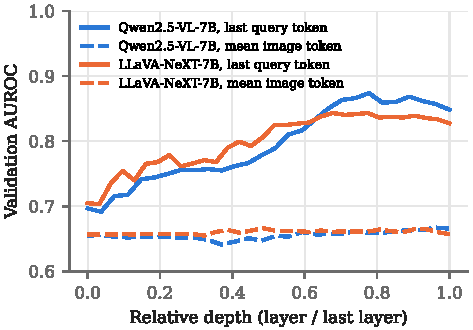
\includegraphics[width=\textwidth]{figures/binary_by_layer.pdf}
\column{0.43\textwidth}
\begin{itemize}
\item Last prompt token, building with depth, plateau in the last third
(Qwen best layer 21/28, LLaVA 24/32)
\item Image tokens flat at 0.62--0.68, near the surface baseline
\item Differs from HALP (Qwen best on visual features for photo
hallucination): for charts, the state that has read the question matters
\end{itemize}
\end{columns}
\end{frame}

% ---------------------------------------------------------------------------
\section{Synthetic arm}

\begin{frame}{Making fabrication happen on purpose}
Ask about a category that is \emph{not} on the chart.
\begin{itemize}
\item \textbf{Pilot 1}: 300 bar charts. Same wording twice per chart: ``What is
the value of Mango?'' (shown) vs.\ ``\dots of Guava?'' (missing)
\item \textbf{Pilot 2}: 300 harder charts, 1,800 questions
\begin{itemize}
\item Lookalike pairs (Dubai/Dublin, Eagle/Falcon): chart shows at most one
\item Three families: \emph{value}, \emph{compare}, \emph{neighbor}
(``Which bar is right of Guava?'')
\item Values never multiples of 5, axes up to 200, sparse ticks
\end{itemize}
\end{itemize}
\textbf{Two guards against leakage}
\begin{itemize}
\item Every contrast is \emph{within one question template} (the template alone
predicts the intended type at AUROC 1.000)
\item Outcomes scored from the actual answer, never from what the question was
designed to cause
\end{itemize}
\end{frame}

\begin{frame}{How the models answered}
\begin{columns}[T]
\column{0.52\textwidth}
\small
\begin{tabular}{llcc}
\toprule
& & Qwen & LLaVA \\
\midrule
\multirow{3}{*}{Shown, right} & value & 554/600 & 185/600 \\
& compare & 300/300 & 209/300 \\
& neighbor & 294/300 & 255/300 \\
\midrule
\multirow{3}{*}{Missing, value} & rejected & 15 & 0 \\
& ``0'' & 494 & 232 \\
& fabricated & 91 & 368 \\
\midrule
Missing, compare & fabricated & 37 & 101 \\
Missing, neighbor & fabricated & 300 & 290 \\
\bottomrule
\end{tabular}
\column{0.45\textwidth}
\begin{itemize}
\item \hl{Neither model refuses}: 15/1,200 (Qwen), 0 (LLaVA)
\item Qwen mostly says ``0''; when it invents, it reads the lookalike bar
(asked Dubai, reports Dublin)
\item LLaVA snaps to gridlines (52 $\to$ 50): only 31\% of shown values right
\item ``0'' is treated as a refusal expressed as a number
\end{itemize}
\end{columns}
\vspace{0.5em}
Value template gives four classes: \cls{c} correct, \cls{s} misread,
\cls{f} invented number, \cls{z} ``0''.
\end{frame}

\begin{frame}{Do the models know the bar is missing? Yes.}
\begin{columns}[T]
\column{0.5\textwidth}
\begin{tabular}{lcc}
\toprule
Test AUROC & Qwen & LLaVA \\
\midrule
value & 0.999 & 0.977 \\
compare & 0.991 & 0.959 \\
neighbor & 1.000 & 0.996 \\
\midrule
lookalikes only & 0.98--1.00 & 0.92--0.99 \\
text-only baseline & 0.49--0.52 & 0.49--0.52 \\
image-token probe & 0.500 & 0.500 \\
\bottomrule
\end{tabular}
\column{0.48\textwidth}
\begin{itemize}
\item Both models \hl{represent that the name is missing, then answer anyway}
\item Text-only baseline at chance: every name is shown on some charts
\item Image-token control is exactly 0.500 by construction (image precedes the
question, attention is causal)
\item Early in Qwen (layer 2), later in LLaVA ($\sim$9)
\end{itemize}
\end{columns}
\end{frame}

\begin{frame}{E3: cross-transfer matrix (the central result)}
\centering
\small
\begin{tabular}{l|ccc|ccc}
\toprule
& \multicolumn{3}{c|}{\qwen} & \multicolumn{3}{c}{\llava} \\
Probe (trained on) & \cls{s} vs \cls{c} & \cls{f} vs \cls{c} & \cls{f} vs \cls{z}
& \cls{s} vs \cls{c} & \cls{f} vs \cls{c} & \cls{f} vs \cls{z} \\
\midrule
structural (\cls{s} vs \cls{c}) & \textbf{0.887} & 0.594 & 0.400 & \textbf{0.776} & \hl{0.879} & 0.215 \\
\quad metadata baseline & 0.814 & 0.557 & 0.543 & 0.512 & 0.522 & 0.537 \\
fabrication (\cls{f} vs \cls{c}) & 0.576 & \textbf{1.000} & 0.286 & 0.680 & \textbf{0.988} & 0.243 \\
invented vs.\ zero (\cls{f} vs \cls{z}) & 0.336 & 0.138 & \textbf{0.984} & 0.520 & 0.226 & \textbf{0.986} \\
\bottomrule
\end{tabular}
\vspace{0.8em}
\raggedright
\begin{itemize}
\item \textbf{Qwen: largely type-specific.} Each probe strong on its own task,
weak on the other
\item \textbf{LLaVA: misread probe is not specific.} It fires \emph{more} on
fabrications than on misreads, a general ``not grounded'' direction
\item \textbf{Both:} the ``fabrication'' probe is really a missing-bar detector
(scores ``0'' as high as invented numbers)
\end{itemize}
{\footnotesize 5-fold CV by chart, out-of-fold AUROC, synthetic value questions.}
\end{frame}

\begin{frame}{E3: where the type signals live}
\begin{columns}[c]
\column{0.55\textwidth}
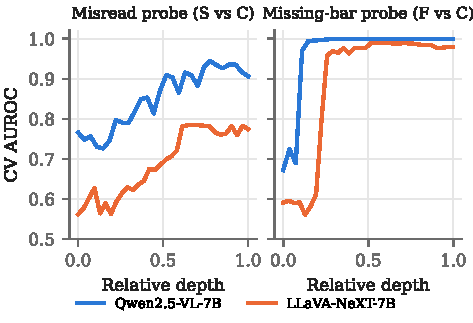
\includegraphics[width=\textwidth]{figures/type_probes_by_layer.pdf}
\column{0.43\textwidth}
\begin{itemize}
\item Missing-bar signal saturates early (Qwen by layer 3, LLaVA $\sim$8)
\item Misread signal builds gradually, peaks in the last third
\item Invented-vs-``0'' only in the last layers: reads out the answer about to
be produced, not an early warning
\end{itemize}
\end{columns}
\end{frame}

% ---------------------------------------------------------------------------
\section{Where we stand}

\begin{frame}{Verdict so far}
\textbf{Hypothesis: supported for Qwen, partly for LLaVA.}
\begin{itemize}
\item \qwen: misread and missing-bar states are linearly distinguishable, each
probe largely blind to the other type
\item \llava: missing-bar signal is specific, but the misread probe captures a
general lack of grounding; a one-number chart feature (distance to nearest
gridline) predicts its misreads at 0.852, above the probe
\end{itemize}
\vspace{0.5em}
\textbf{Caveats we already know about}
\begin{itemize}
\item On synthetic data, ``fabrication'' and ``missing category'' coincide
\item Qwen has only 46 synthetic misreads; the ChartQA structural probe has 13
test positives and no surface baseline yet
\item Labels are from one LLM annotator, human $\kappa$ check pending
\end{itemize}
\end{frame}

\begin{frame}{Status and next steps}
\begin{columns}[T]
\column{0.48\textwidth}
\textbf{Done}
\begin{itemize}\small
\item Inference and full-depth caches: both models, ChartQA test, val\_human
(Qwen), both pilots
\item 317 Qwen error labels
\item E1 both models; E3 both models
\end{itemize}
\textbf{Coded, waiting for the cluster}\\
{\small (maintenance; the activation caches live there)}
\begin{itemize}\small
\item Synthetic $\to$ ChartQA transfer: does the synthetic misread probe flag the
71 real misreads?
\item \cls{computation} as a third class vs.\ misreads
\item E4 intervention matrix
\end{itemize}
\column{0.5\textwidth}
\textbf{Timeline}
\begin{itemize}\small
\item \textbf{Oct 1--8}: human $\kappa$ on 200 items; LLaVA's 1,178 error
labels; residualised probes (E2)
\item \textbf{Oct 1--15}: E4 repairs (crop, verify prompt, abstain) on
synthetic items, both models
\item \textbf{Oct 16--25}: E5 controller; risk--coverage vs.\ binary selective
prediction and the oracle
\item \textbf{Oct 26--31}: final report
\end{itemize}
\end{columns}
\end{frame}

\begin{frame}{Where we would like guidance}
\begin{enumerate}
\item \textbf{Fabrication definition.} Is ``asked about a missing category'' an
acceptable operationalisation, or should we add out-of-range quantities so
fabrication is not identical to absence?
\item \textbf{Taxonomy.} Should \cls{computation} become a third type in the
hypothesis, given it is the largest real error class?
\item \textbf{Annotation.} Is an LLM annotator acceptable if it passes a
two-person human agreement check ($\kappa > 0.6$ on 200 items)?
\item \textbf{Label noise.} Should the 112 \cls{not\_an\_error} items be
re-scored as correct in every experiment, or reported both ways?
\item \textbf{Scope of E4/E5.} Is running the repairs on synthetic charts only
(where bar geometry is known) enough, or do we need ChartQA repairs too?
\end{enumerate}
\end{frame}

\begin{frame}[standout]
Thank you
\end{frame}

\end{document}
